\documentclass[11pt]{beamer}
\usetheme{bars}
\usepackage{xcolor}
\usepackage[utf8x]{inputenc}
\usepackage{ucs}
\usepackage[spanish]{babel}
\usepackage{amsmath}
\usepackage{amsfonts}
\usepackage{multirow}
\usepackage{amssymb}
\usepackage{fancybox}
\usepackage{multicol}
\usepackage{graphicx}
\usepackage{multicol}
\graphicspath{{Figures/}}
%\setbeamercovered{transparent} 
\definecolor{colorZ}{RGB}{0,60,127}
\usecolortheme[RGB={0,60,127}]{structure}
\setbeamertemplate{navigation symbols}{}
\setbeamercolor{mycolor}{bg=colorZ,fg=white}
\defbeamertemplate*{footline}{shadow theme}{%
\leavevmode%
\hbox{\begin{beamercolorbox}[wd=.5\paperwidth,ht=2.5ex,dp=1.125ex,leftskip=.3cm plus1fil,rightskip=.3cm]{author in head/foot}%
    \usebeamerfont{author in head/foot}\hfill\insertshortauthor
\end{beamercolorbox}%
\begin{beamercolorbox}[wd=.43\paperwidth,ht=2.5ex,dp=1.125ex,leftskip=.3cm,rightskip=.3cm plus1fil]{title in head/foot}%
    \usebeamerfont{title in head/foot}\insertshorttitle\hfill%
\end{beamercolorbox}%
\begin{beamercolorbox}[wd=.07\paperwidth,ht=2.5ex,dp=1.125ex,leftskip=.1cm,rightskip=.1cm plus1fil]{mycolor}%
\hfill\insertframenumber\,/\,\inserttotalframenumber
\end{beamercolorbox}}%
\vskip0pt%
}
\author[Daniel Osorio]{\vspace*{-0.55cm}\\\normalsize{\scriptsize{Presented by:}\\\normalsize{\textbf{Daniel Camilo Osorio Hurtado}}}\\\scriptsize{in partial fulfillment of requirements for the degree of} \normalsize{\\\textbf{Master in Bioinformatics}\newline \newline Advisors: \textbf{Janneth Gonzalez PhD.} and \textbf{Andrés Pinzon PhD.}}\\\scriptsize{Bioinformatics and Computational Systems Biology Lab}}
\title[Bioinformatics Master Thesis]{Identifying proteins and metabolic pathways associated to the neuroprotective response mediated by tibolone in astrocytes under an induced inflammatory model}
\date[]{\scriptsize{\vspace{-1.1cm}\\\includegraphics[scale=.1]{UN}\\\textbf{Universidad Nacional de Colombia\\ Engineering Faculty - Department of Systems and Industrial Engineering\\Bogotá, Colombia}}}
\begin{document}
\maketitle
\section{Introduction}
%\begin{frame}{Neuroinflammation}
%\begin{center}
%\includegraphics[width=9.5cm]{BInflam}
%\end{center}
%\begin{center}
%\fcolorbox{cyan}{cyan}{{Neurodegenerative diseases}}
%\fcolorbox{cyan}{cyan}{{Cardiovascular events}}
%\fcolorbox{cyan}{cyan}{{Stress}}
%\fcolorbox{cyan}{cyan}{{Smoke}}
%\fcolorbox{red}{red}{{Obesity (Over Nutrition or Caloric Excess)}}
%\end{center}
%\end{frame}
%\begin{frame}{Metabolic Inflammation or Metainflammation}
%\begin{center}
%\fcolorbox{black}{black}{\textcolor{white}{$\blacktriangledown$ Leptine}} + 
%\fcolorbox{black}{black}{\textcolor{white}{$\blacktriangledown$ Insuline}} $\rightarrow$ \fcolorbox{red}{red}{\textcolor{white}{$\blacktriangle$ IKK$\beta$}} + \fcolorbox{red}{red}{\textcolor{white}{$\blacktriangle$ NF$\kappa\beta$}} 
%\end{center}
%\pause
%\begin{center}
%\fcolorbox{blue}{blue}{\textcolor{white}{$\blacktriangle$ Endoplasmic reticulum stress}} $\rightarrow$ \fcolorbox{blue}{blue}{\textcolor{white}{$\blacktriangle$ UPR}}
%\end{center}
%\begin{center}
%\fcolorbox{green}{green}{{$\blacktriangle$ Reactive C Protein Ligands}}  + \fcolorbox{green}{green}{{$\blacktriangle$ TNF$\alpha$}} + \fcolorbox{green}{green}{{$\blacktriangle$ IL6}} + \fcolorbox{green}{green}{{$\blacktriangle$ ROS}} 
%\end{center}
%\end{frame}
%\begin{frame}{Astrocytes Metabolic Functions}
%\begin{center}
%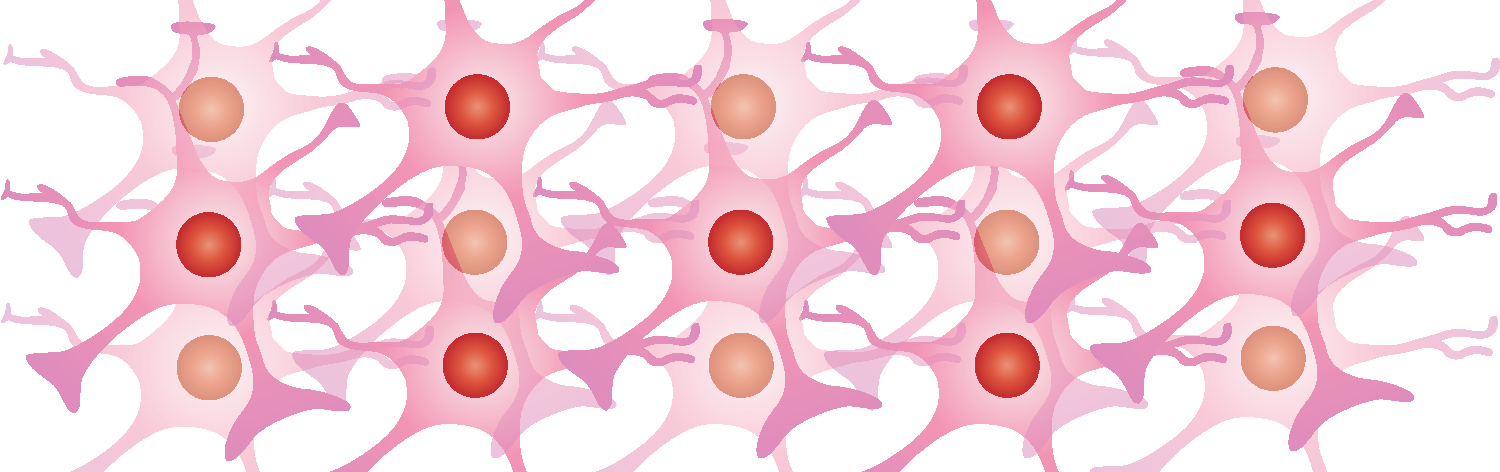
\includegraphics[width=6cm]{GFAP} \pause
%\end{center}
%\begin{center}
%\fcolorbox{yellow}{yellow}{{K$^{+}$ Membrane Potential}} \pause
%\fcolorbox{yellow}{yellow}{{Ca$^{+2}$ signaling}} \pause
%\fcolorbox{yellow}{yellow}{{Lactate release}} \pause
%\fcolorbox{yellow}{yellow}{{[Dopa], [Glu], [GABA], [Gly] and [Cys] regulator}} \pause
%\fcolorbox{yellow}{yellow}{{pH maintenance}} \pause
%\fcolorbox{yellow}{yellow}{{ROS detox}} \pause
%\fcolorbox{yellow}{yellow}{{Gln, ATP and D-serine release}}
%\end{center}
%\end{frame}
%\begin{frame}{What effects does tibolone have on Astrocytic inflammatory scenarios?}
%\begin{center}
%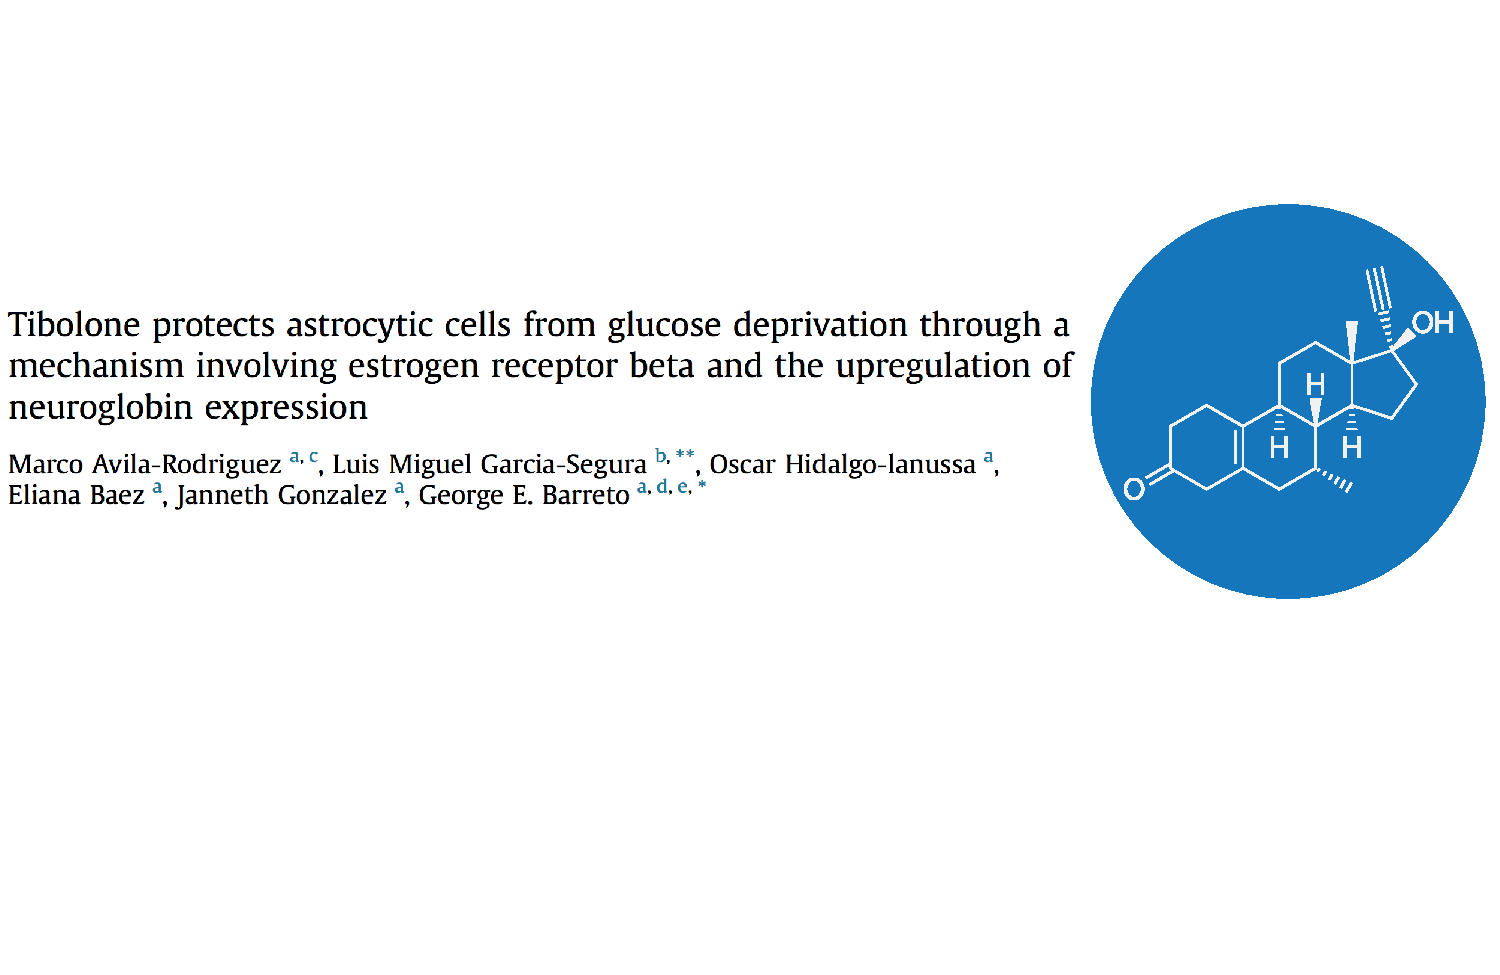
\includegraphics[width=\textwidth]{Tibolone}
%\end{center}
%\end{frame}
\section{Objectives and Methods}
\begin{frame}{Objectives:}
To identify proteins and metabolic pathways involved in the neuroprotective effects of tibolone in human astrocytes based in metabolic scenarios comparation we set:
\begin{itemize}
\item Build a tissue specific computational model of astrocytes metabolism using gene expression data integration.
\item Evaluate the effects caused by the increase of free fatty acids and tibolone presence in astrocytes metabolism.
\item Determine metabolic pathways and relevant functional products in response to steroid tibolone through systems biology approximations.
\item Evaluate the importance of proteins and metabolic pathways previously identified on the dynamics of the metabolic model.
\end{itemize}
\end{frame}
\begin{frame}
\begin{block}{\textbf{OBJECTIVE 1:}}
\begin{center}
Build a tissue specific computational model of \\astrocytes metabolism using gene expression data integration.
\end{center}\end{block}
\end{frame}
\begin{frame}{Healthy Human Astrocytes Gene Expression Data}
\begin{center}
\begin{multicols}{2}
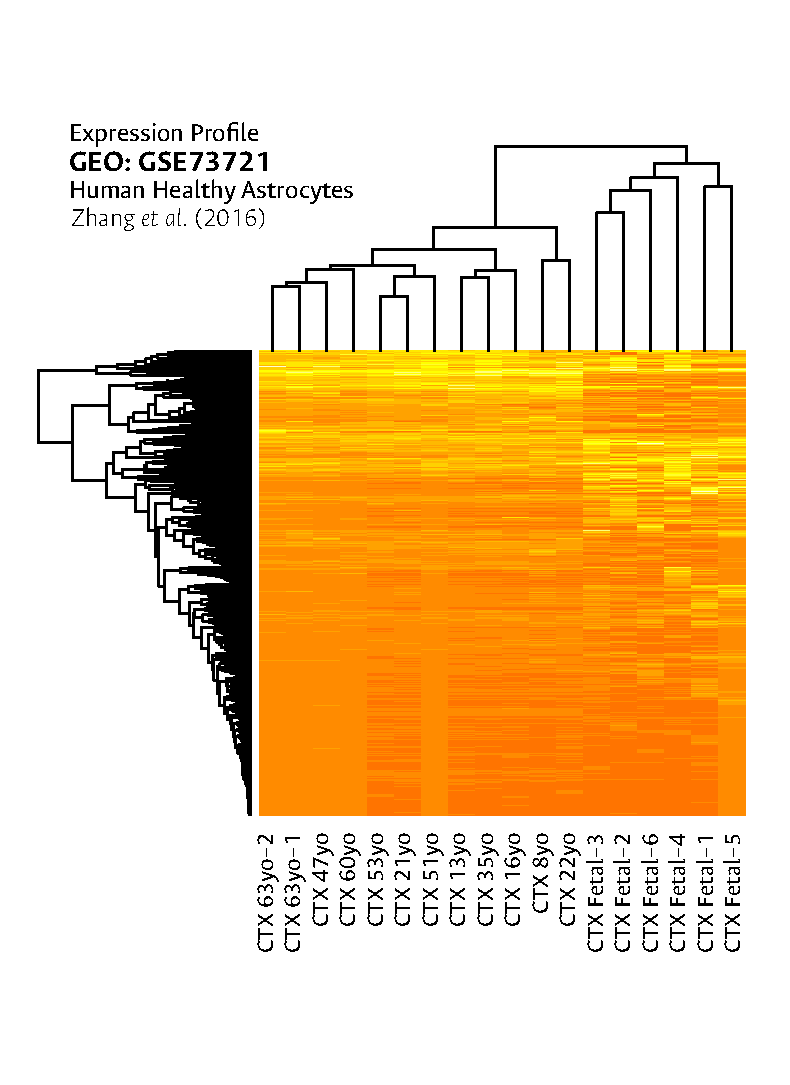
\includegraphics[width=5cm]{GE}\\
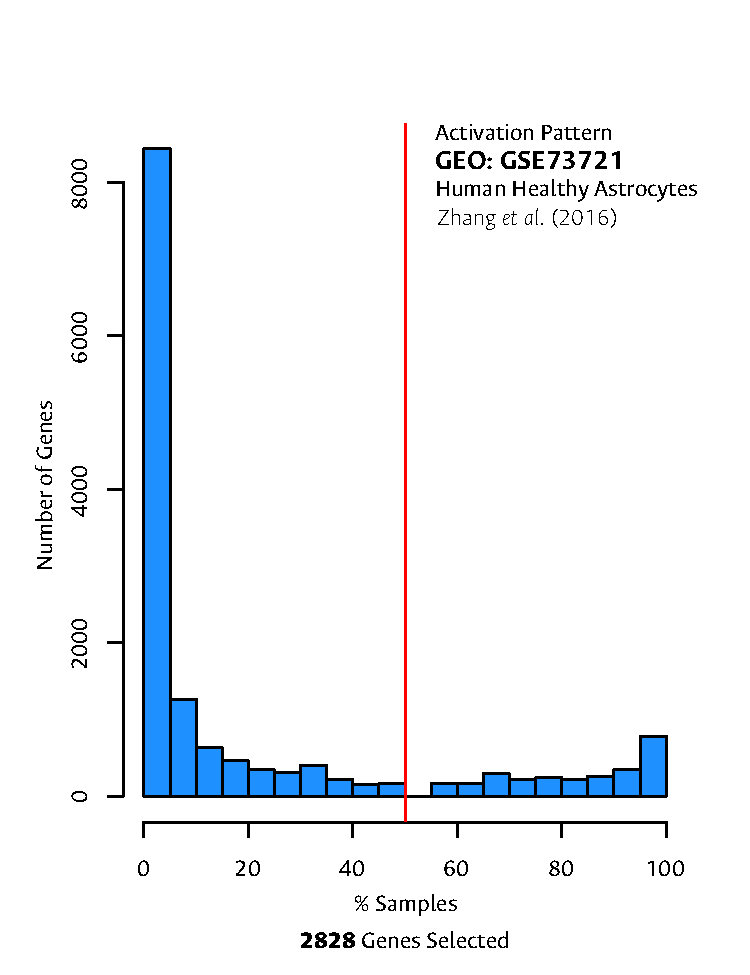
\includegraphics[width=5cm]{ActiveGenes}
\end{multicols}
\end{center}
\end{frame}
\begin{frame}{Mapping Reactions}
\begin{center}
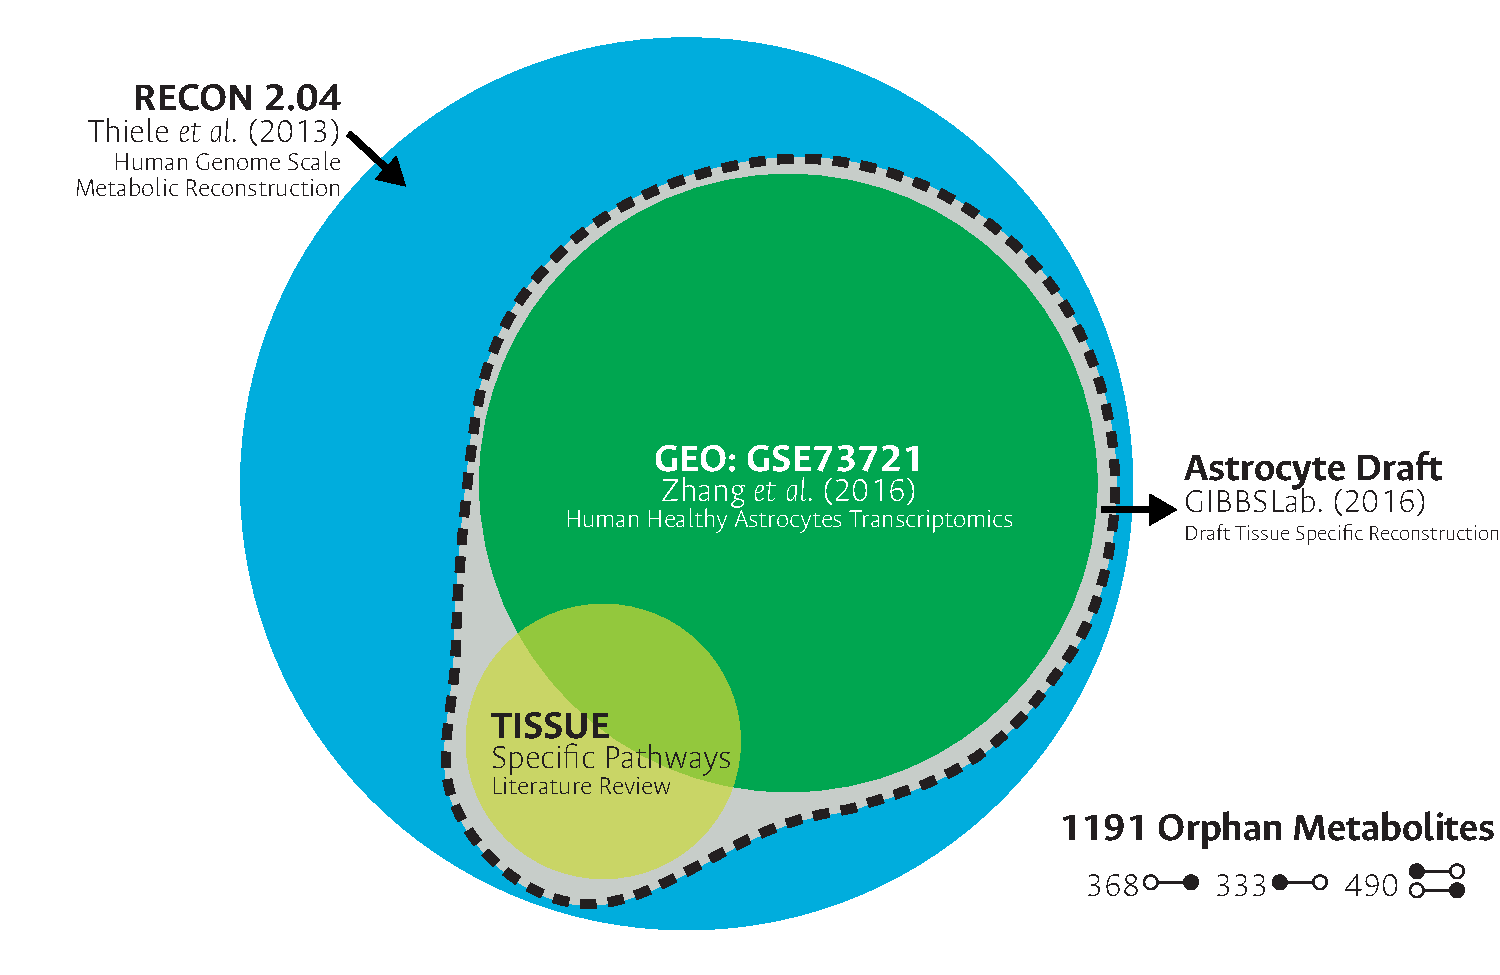
\includegraphics[width=\textwidth]{TSR}
\end{center}
\end{frame}
\begin{frame}{Gap-Find and Gap-Fill Available Algorithms}
\begin{center}
\begin{tabular}{r|c|p{3.7cm}}
\hline
\textbf{ALGORITHM}&\textbf{ENVIRONMENT}&\textbf{HOW IT WORKS}\\
\hline
\hline
\multirow{2}{*}{SMILEY}&\multirow{2}{*}{Python - OpenSource}&· Optimization based.\\
&&· \textbf{Fills one metabolite \emph{per time}}.\\
\hline
\multirow{2}{*}{gap-Find/Fill}&\multirow{2}{*}{GAMS - OpenSource}&· Optimization based.\\
&&· \textbf{Makes several \emph{intra model modifications}}.\\
\hline
\multirow{2}{*}{growMatch}&\multirow{2}{*}{Python - OpenSource}&· Optimization based.\\
&&· \textbf{Fills one objective function \emph{per time}}.\\
\hline
\multirow{2}{*}{fastGapFill}&\multirow{2}{*}{MATLAB - \textbf{Privative}}&· Optimization based.\\
&&· Multiobjective.\\
\hline
\end{tabular}
\end{center}
\end{frame}
\begin{frame}{Finding and Filling Gaps}
\begin{center}
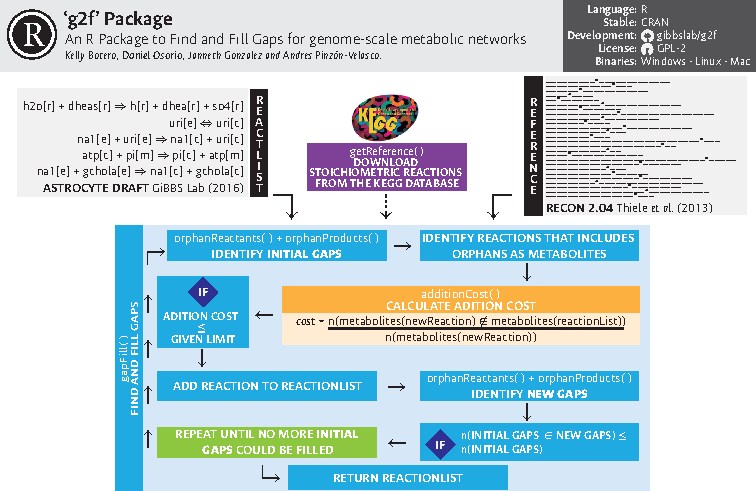
\includegraphics[width=\textwidth]{g2f}
\end{center}
\end{frame}
\begin{frame}{Syntax, Mass-Charge Validation and SBML files}
\begin{center}
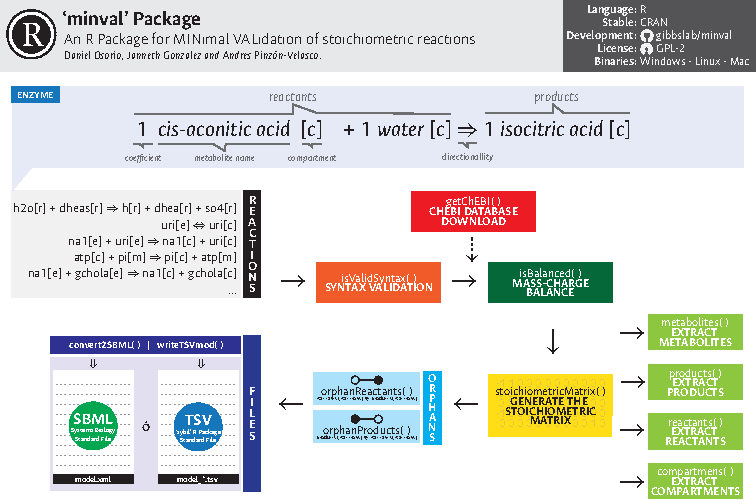
\includegraphics[width=\textwidth]{minval}
\end{center}
\end{frame}
\begin{frame}{Metabolic Model Debugging}
\begin{center}
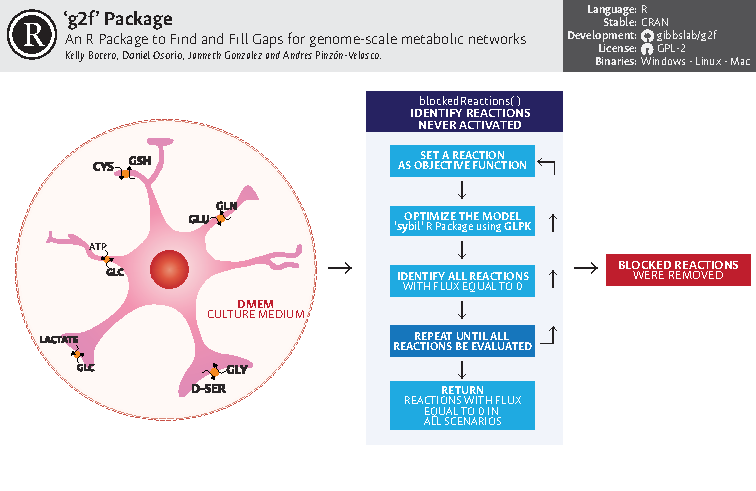
\includegraphics[width=\textwidth]{Debug}
\end{center}
\end{frame}
\begin{frame}{Gene Expression Integration Available Methods}
\begin{center}
\begin{tabular}{r|p{3cm}|p{4.7cm}}
\hline
\textbf{METHOD}&\textbf{ENVIRONMENT}&\textbf{HOW IT WORKS}\\
\hline
\hline
\multirow{2}{*}{GIMME}&\multirow{2}{*}{\parbox{3cm}{\centering{MATLAB  \textbf{Privative}}}}&·{\footnotesize \textbf{Binary Disctretization}}\\
&&·{\footnotesize  \textbf{Ensures flux for a selected objective function}}\\
\hline
\multirow{2}{*}{iMAT}&\multirow{2}{*}{\parbox{3cm}{\centering{MATLAB  \textbf{Privative}}}}&· {\footnotesize Integration proportional to gene-expression (H, M and L categorization)} \\
&&· {\footnotesize Not objective function required} \\
\hline
\multirow{2}{*}{E-FLUX}&\multirow{2}{*}{\textbf{Not implemented}}&· {\footnotesize \textbf{Requires a user-given threshold}}\\
&&· {\footnotesize  Continuous Integration}\\
\hline
\multirow{2}{*}{PROM}&\multirow{2}{*}{\parbox{3cm}{\centering{MATLAB  \textbf{Privative}}}}&·{\footnotesize \textbf{Requires a user-given regulatory network}}\\
&&· {\footnotesize Constraints are setting according to the associated transcript. factor}\\
\hline
\end{tabular}
\end{center}
\end{frame}
\begin{frame}{Constraining the Metabolic Model}
\begin{center}
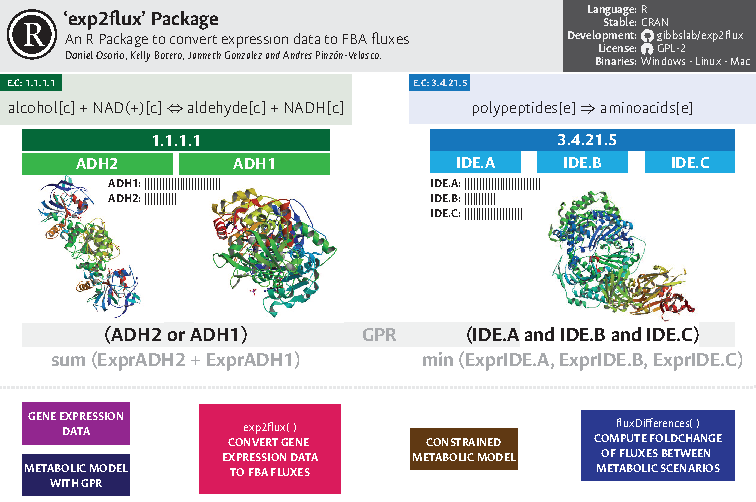
\includegraphics[width=\textwidth]{exp2flux}
\end{center}
\end{frame}
\begin{frame}{Human Healthy Mature Astrocyte Model}
\begin{center}
\includegraphics[width=\textwidth]{Ages}
\end{center}
\end{frame}
\begin{frame}
\begin{block}{\textbf{OBJECTIVE 2:}}
\begin{center}
Evaluate the effects caused by the increase of free fatty acids and tibolone presence in astrocytes metabolism.\end{center}\end{block}
\end{frame}
\begin{frame}{Metabolic Scenarios}
\begin{center}
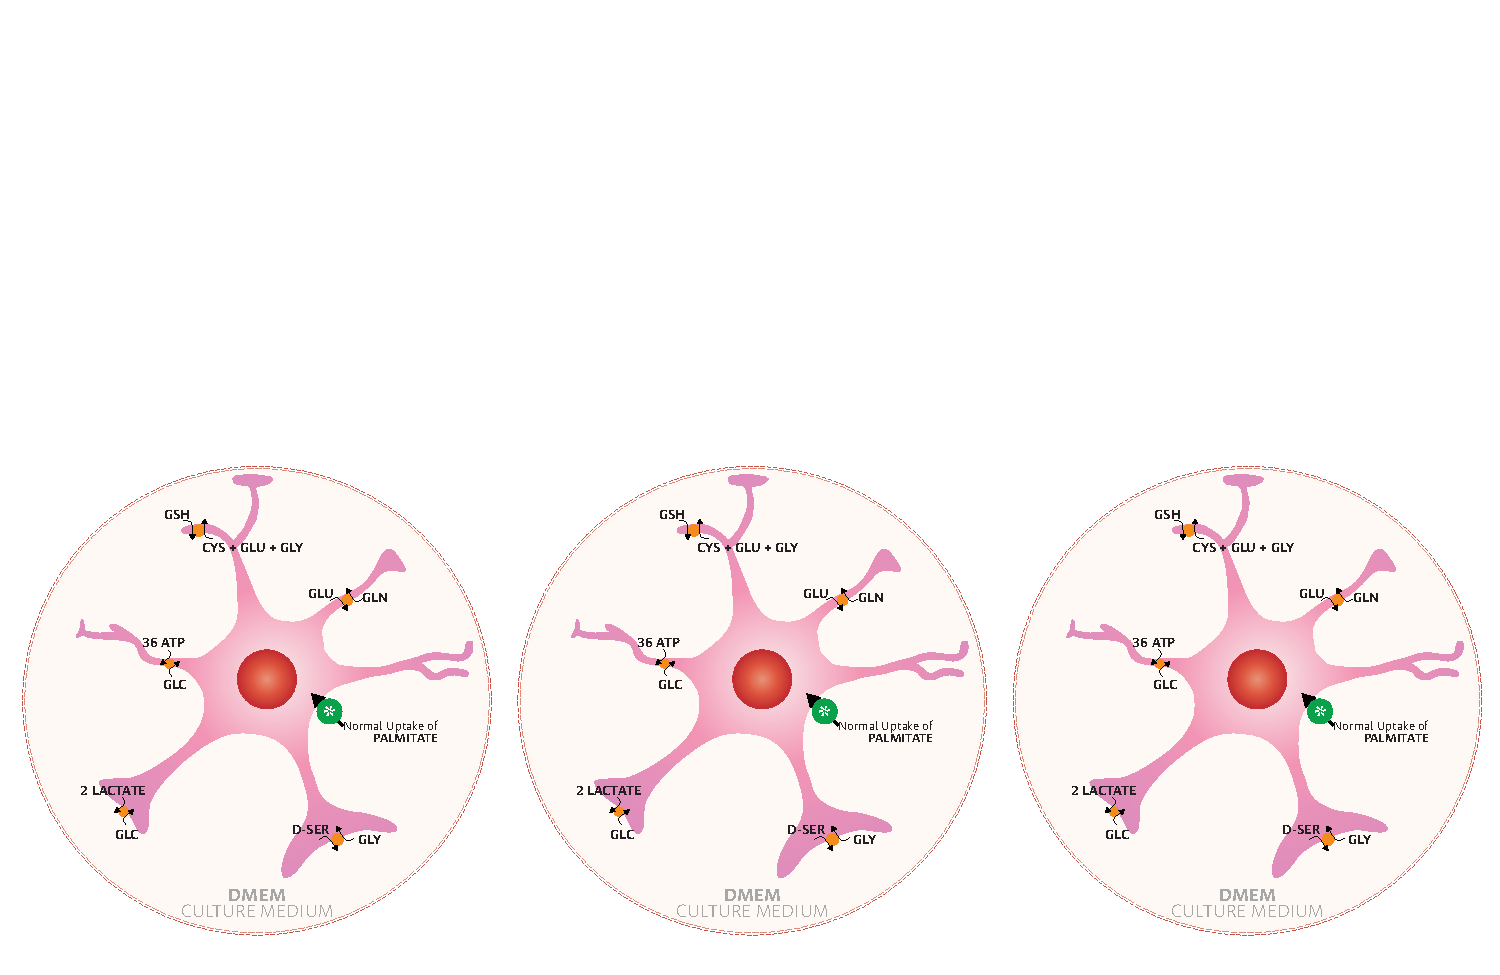
\includegraphics[width=\textwidth]{Healthy}\\
\textbf{MAIN OBJECTIVE FUNCTION:}\\Generic Human Biomass Reaction included in RECON 2.04 \\(Thiele \textit{et al.}, 2013)
\end{center}
\end{frame}
\begin{frame}{Inflamed Metabolic Scenario}
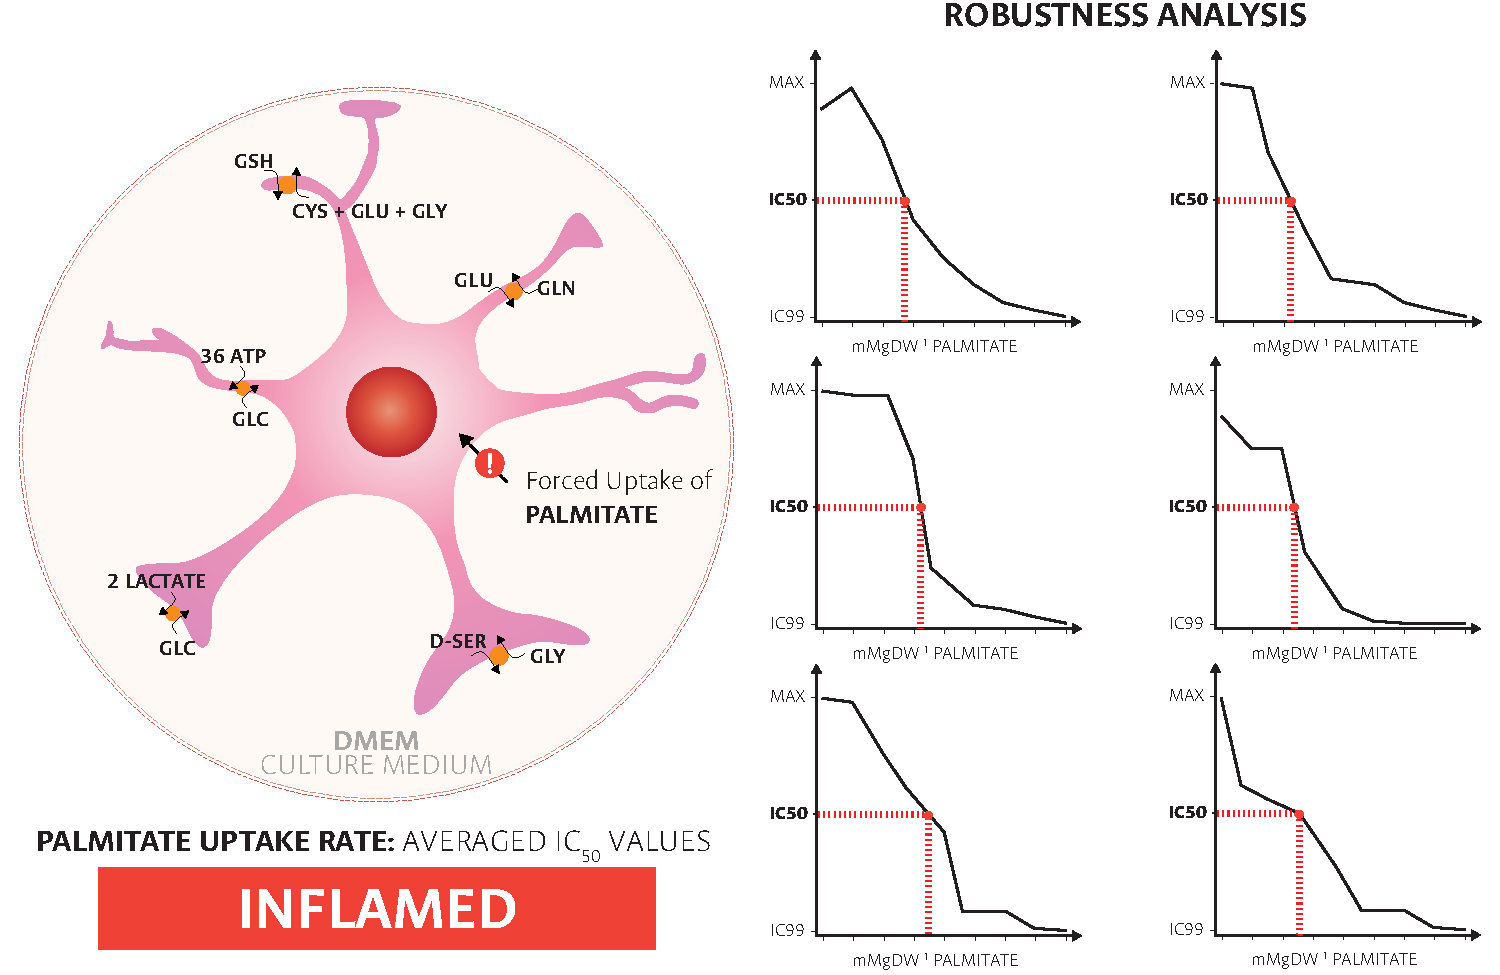
\includegraphics[width=\textwidth]{Inflamed}
\end{frame}
\begin{frame}{Medicated Metabolic Scenario}
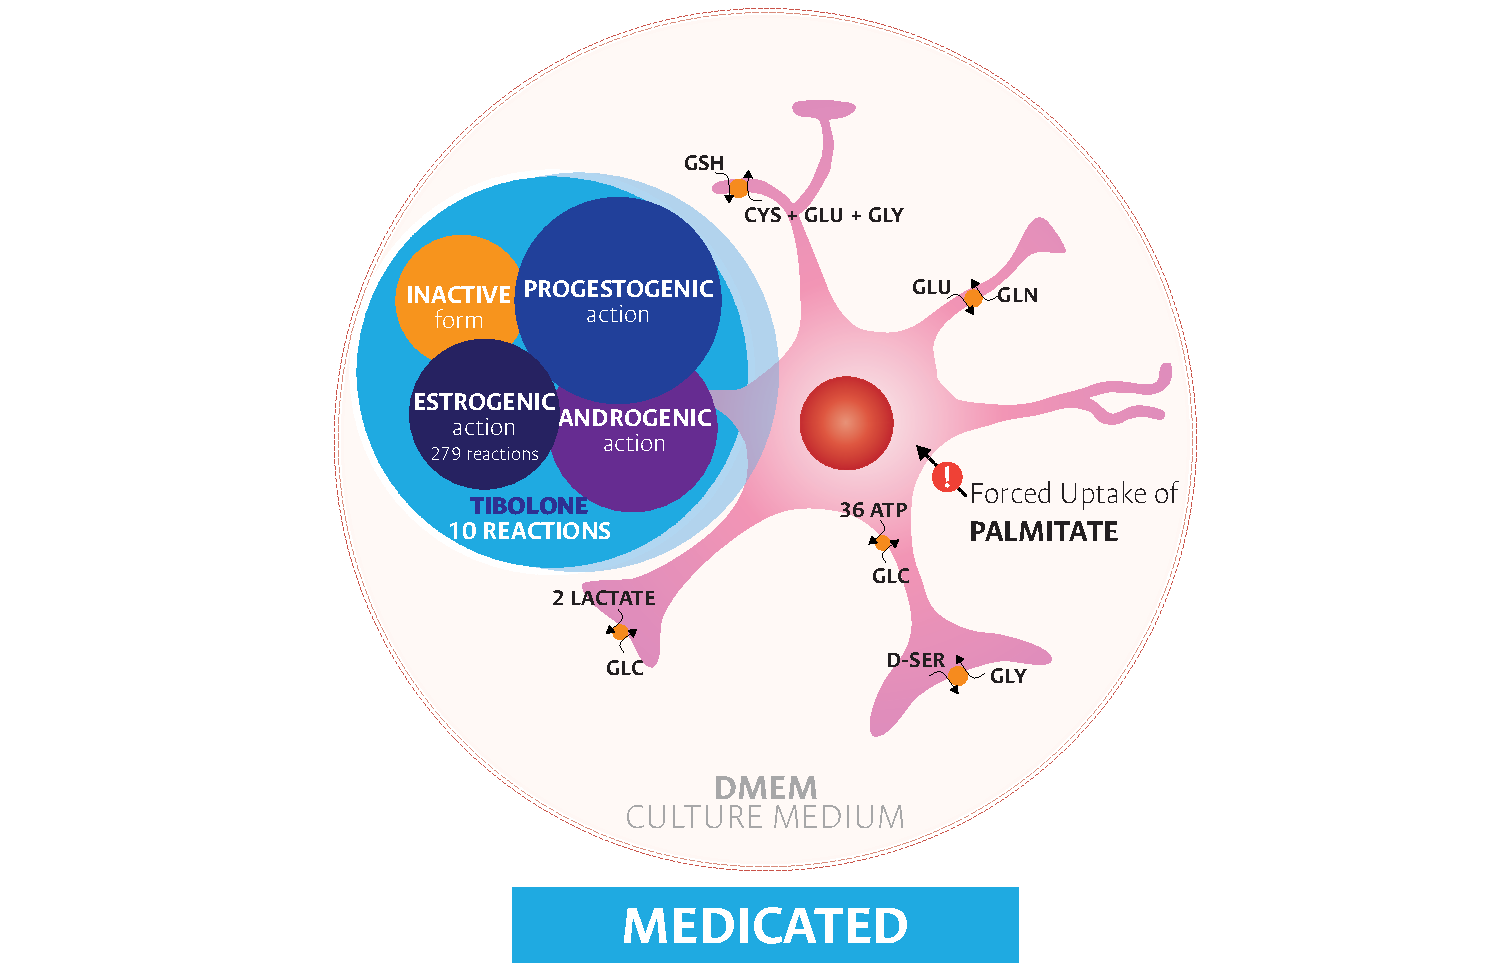
\includegraphics[width=\textwidth]{Medicated}
\end{frame}
\begin{frame}
\begin{block}{\textbf{OBJECTIVE 3:}}
\begin{center}
Determine metabolic pathways and relevant functional products in response to steroid tibolone through systems biology approximations.\end{center}\end{block}
\end{frame}
\begin{frame}{Metabolic Pathways Activation Pattern Changes}
\begin{center}
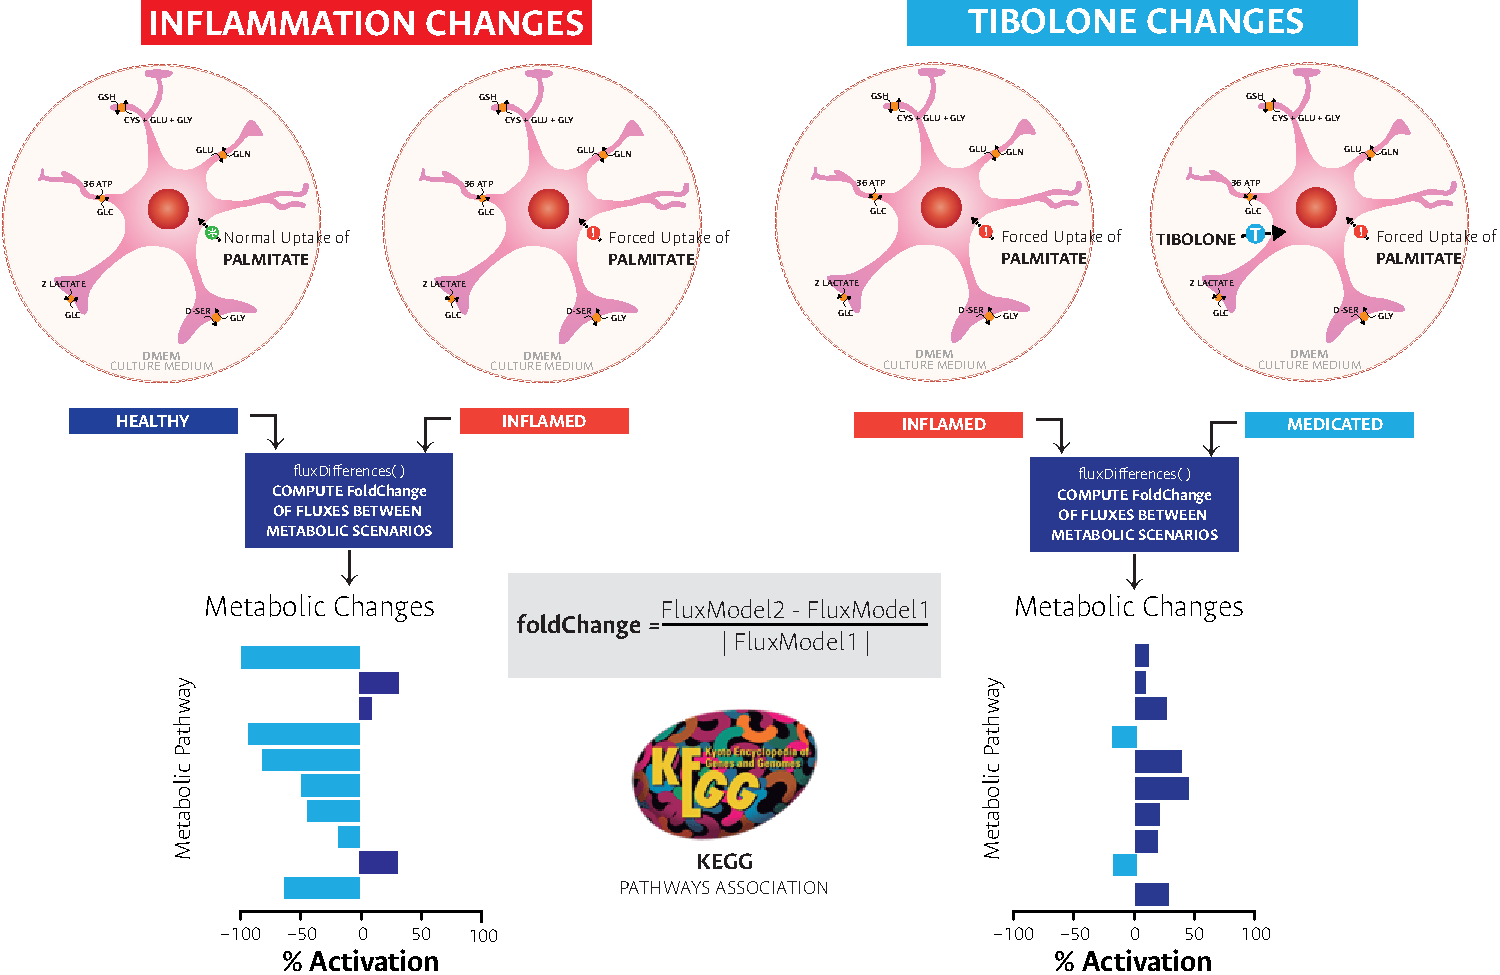
\includegraphics[width=\textwidth]{FluxDifferenes}
\end{center}
\end{frame}
\begin{frame}{Changes in Metabolites Production}
\begin{center}
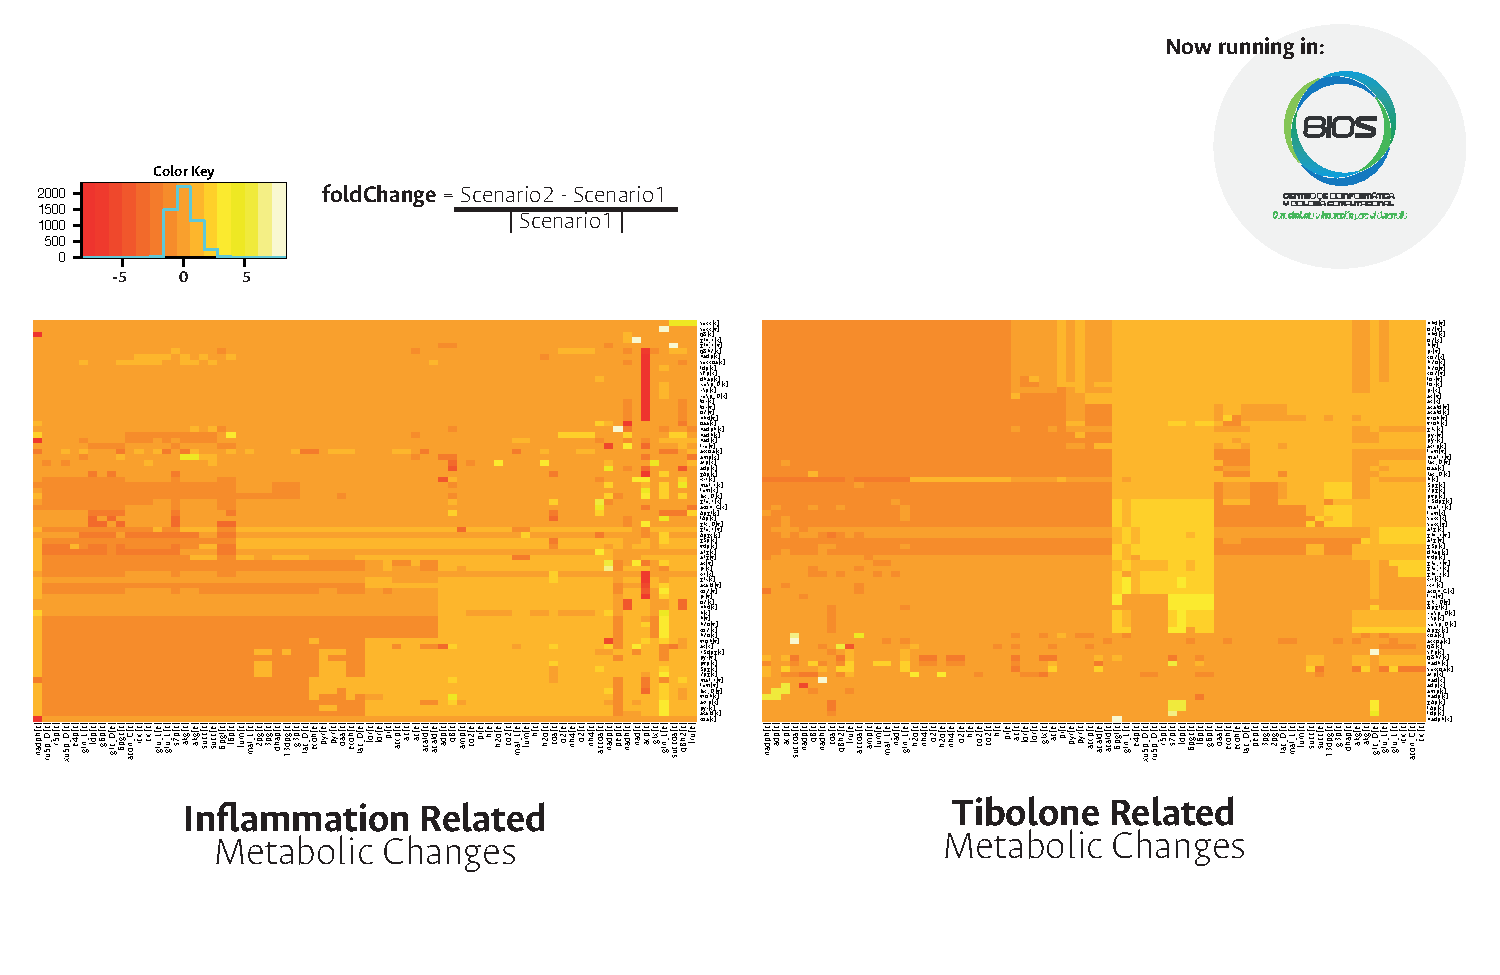
\includegraphics[width=\textwidth]{MetChanges}
\end{center}
\end{frame}
\begin{frame}
\begin{block}{\textbf{OBJECTIVE 4:}}
\begin{center}
Evaluate the importance of proteins and metabolic pathways previously identified on the dynamics of the metabolic model.\end{center}\end{block}
\end{frame}
\begin{frame}
\begin{center}
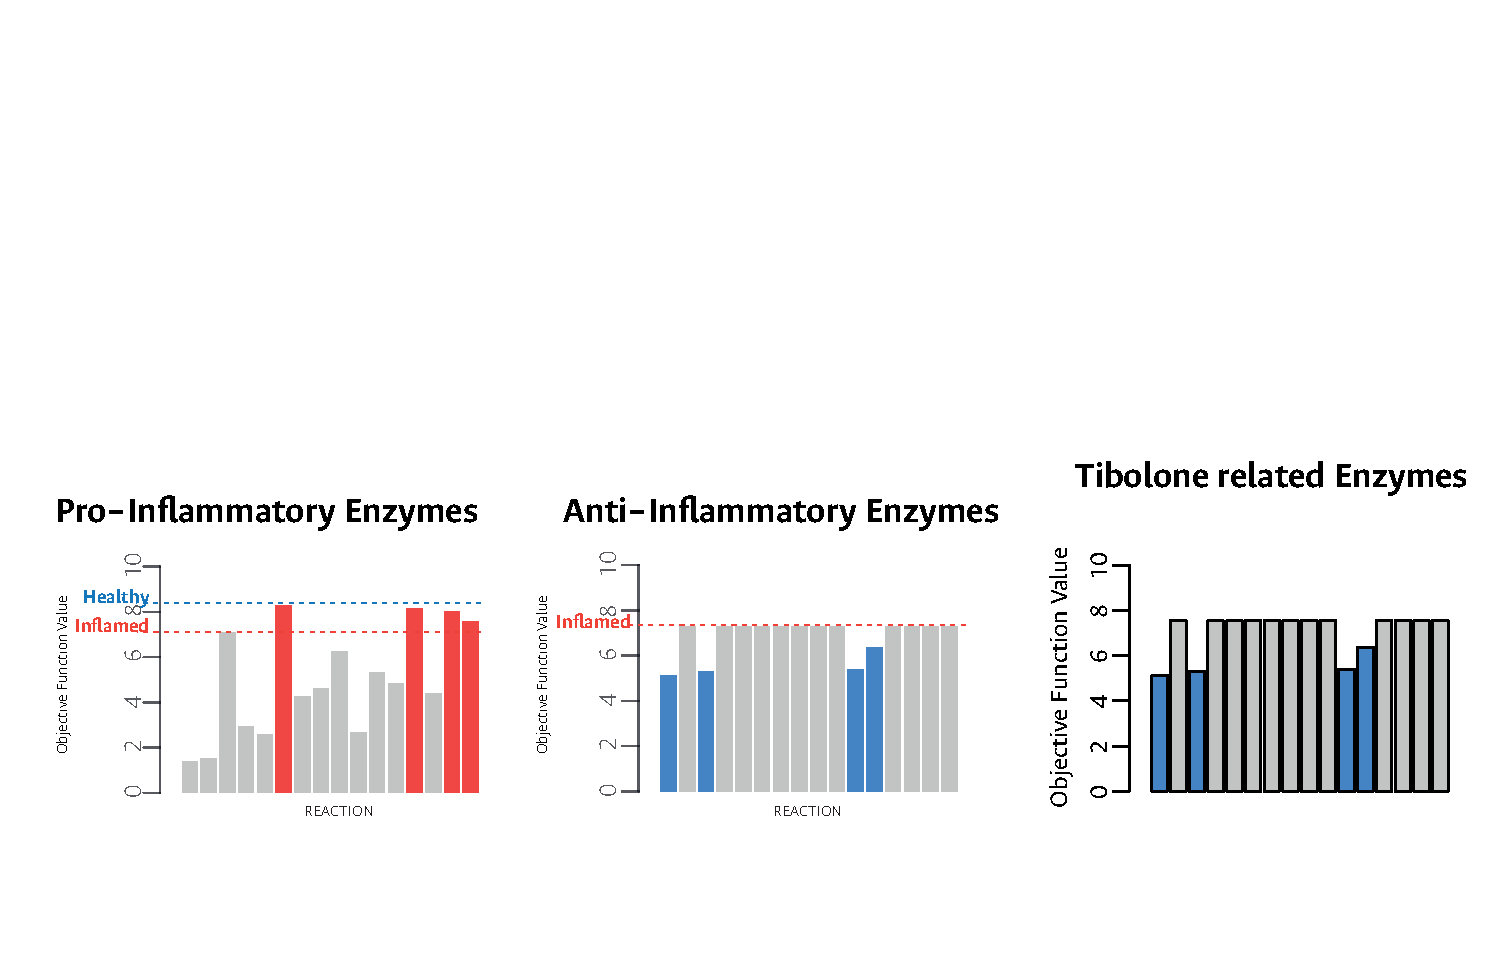
\includegraphics[width=\textwidth]{Networks}
\end{center}
\end{frame}
\section{Results}
\begin{frame}{Software Packages}
\begin{center}

\includegraphics[width=\textwidth]{SPackages}
\end{center}
\end{frame}
\begin{frame}{Astrocyte Model}
\begin{center}
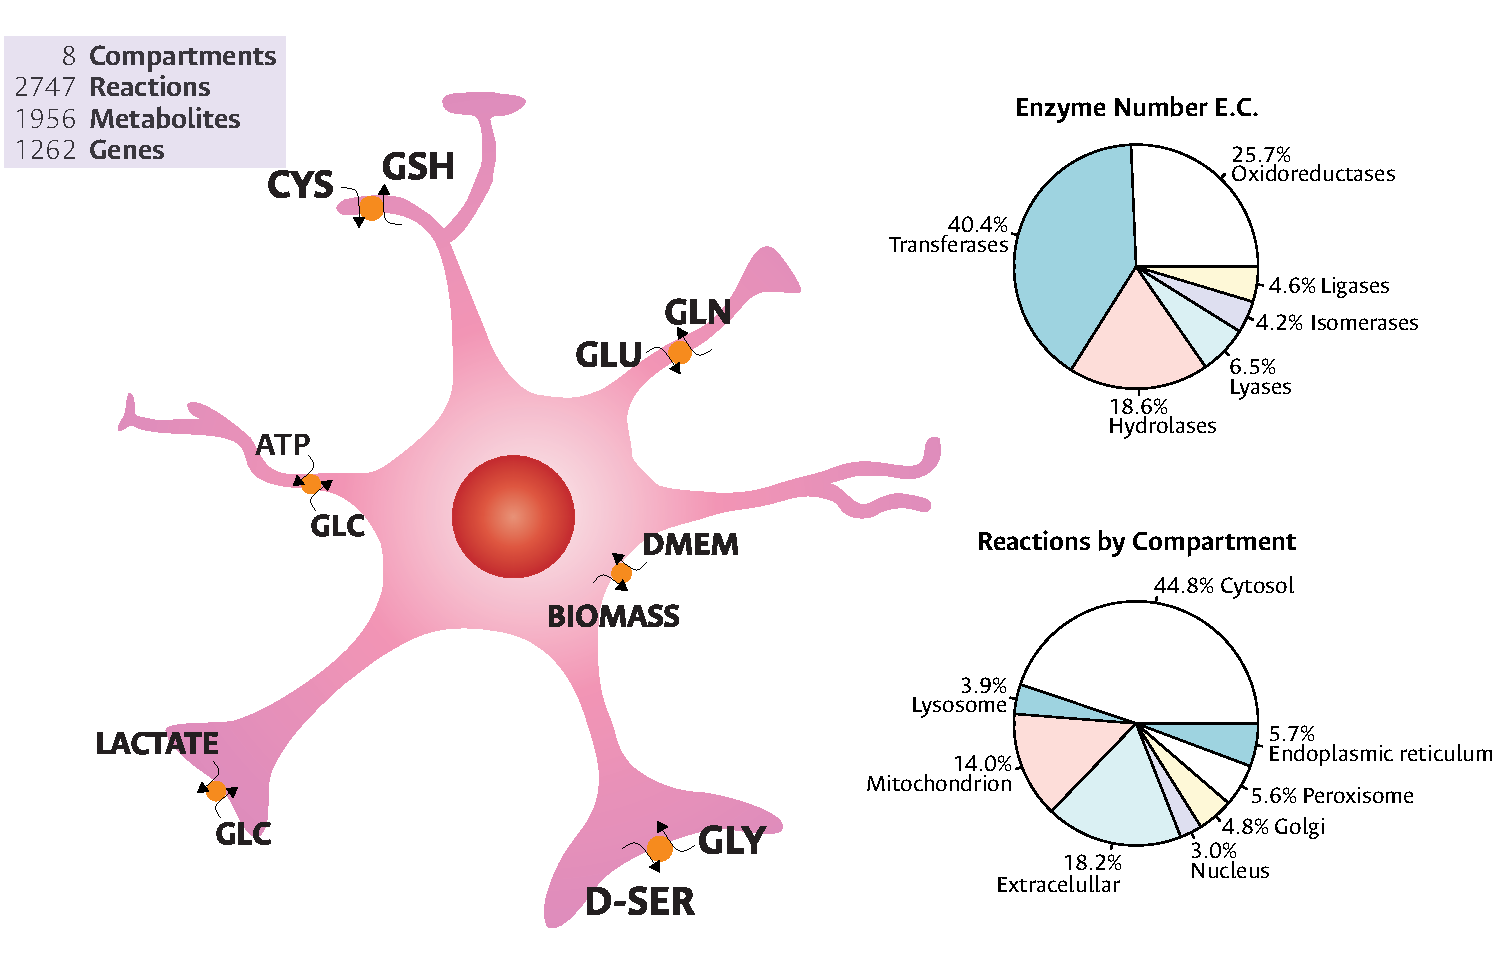
\includegraphics[width=\textwidth]{Astrocyte}
\end{center}
\end{frame}
\begin{frame}{Age Related Metabolic Changes in Astrocytes}
\begin{center}
\includegraphics[width=\textwidth]{Astrocyte_MetabolicChanges}
\end{center}
\end{frame}
\begin{frame}{IC$_{50}$ = 0.208 $\pm$ 0.024 mMgDW$^{-1}$h$^{-1}$}
\begin{center}
\includegraphics[width=\textwidth]{IC50}
\end{center}
\end{frame}
\begin{frame}{Inflammation Related Metabolic Changes in Astrocytes}
\begin{center}
\includegraphics[width=\textwidth]{Healthy2Inflammated}
\end{center}
\end{frame}
\begin{frame}{Gliotransmitters Release Rate}
\begin{center}
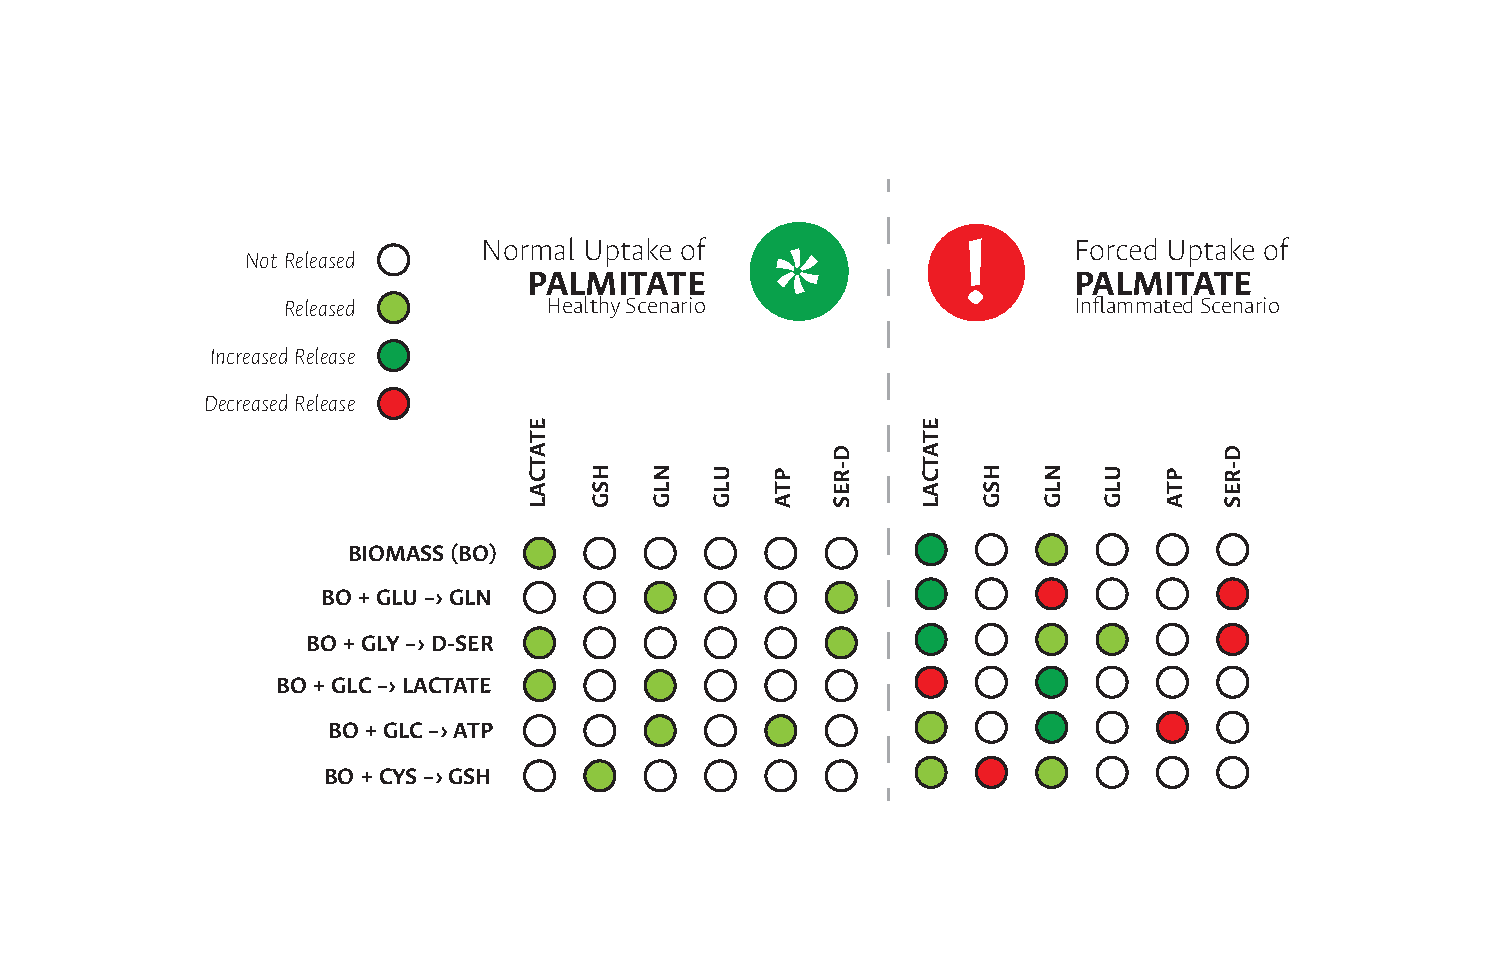
\includegraphics[width=\textwidth]{GTi}
\end{center}
\end{frame}
\begin{frame}{Tibolone Effects in Inflammated Astrocytes}
\begin{center}
\includegraphics[width=\textwidth]{Effects}
\end{center}
\end{frame}
\begin{frame}{Tibolone Metabolic Changes in Inflammated Astrocytes}
\begin{center}
\includegraphics[width=\textwidth]{Inflammated2Tibolone}
\end{center}
\end{frame}
\begin{frame}{Gliotransmitters Release Rate}
\begin{center}
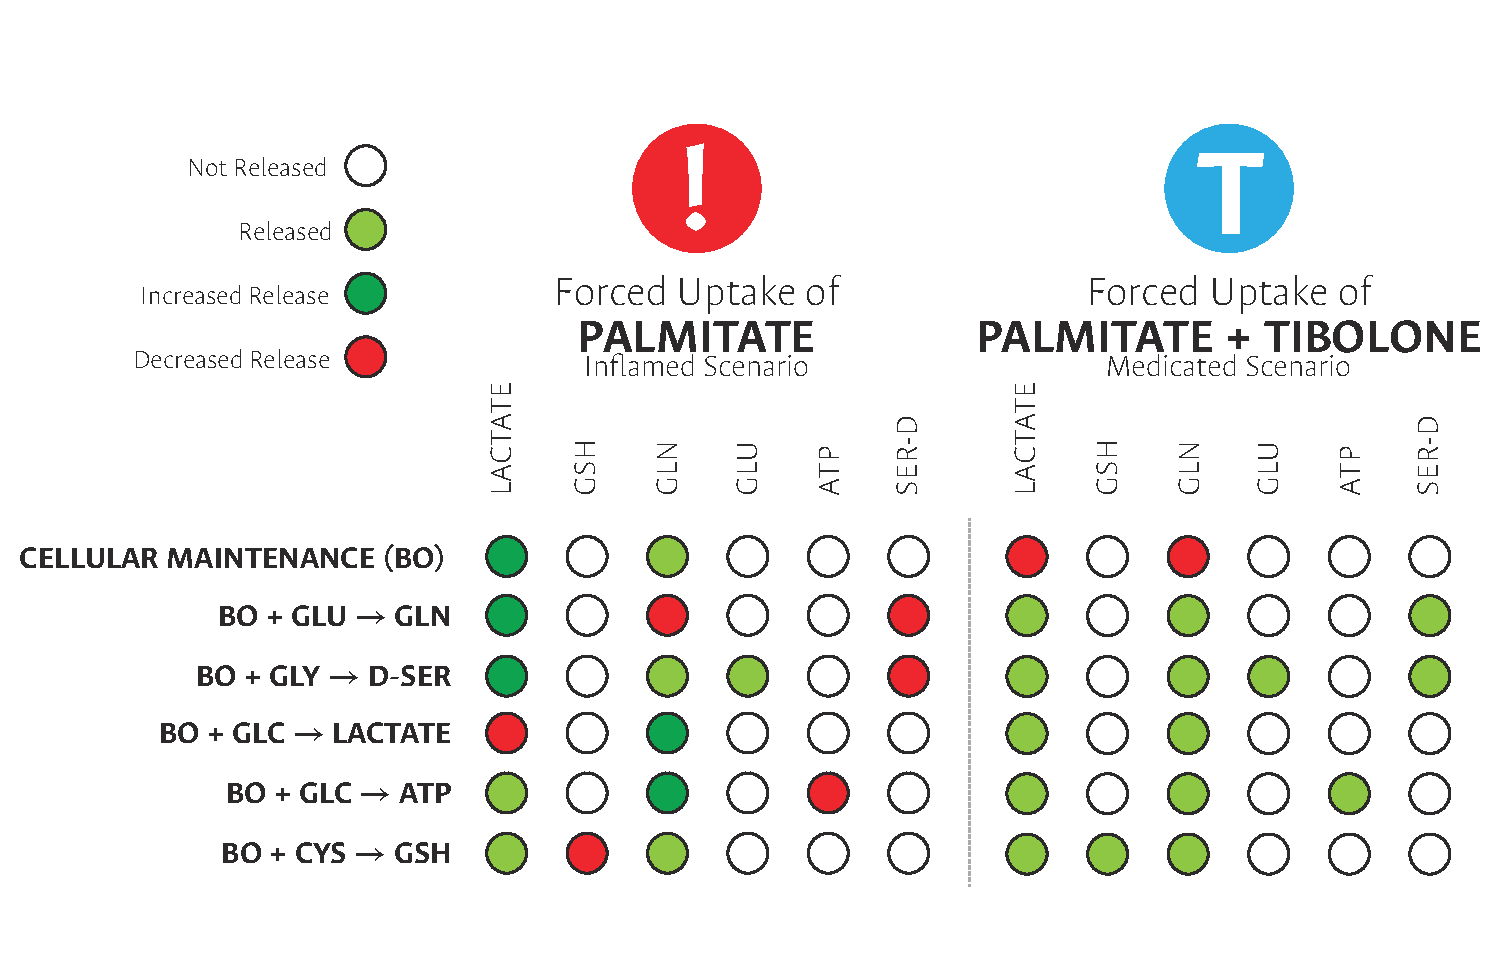
\includegraphics[width=\textwidth]{GTt}
\end{center}
\end{frame}
\begin{frame}{ProInflammatory Enzymes}
\begin{center}
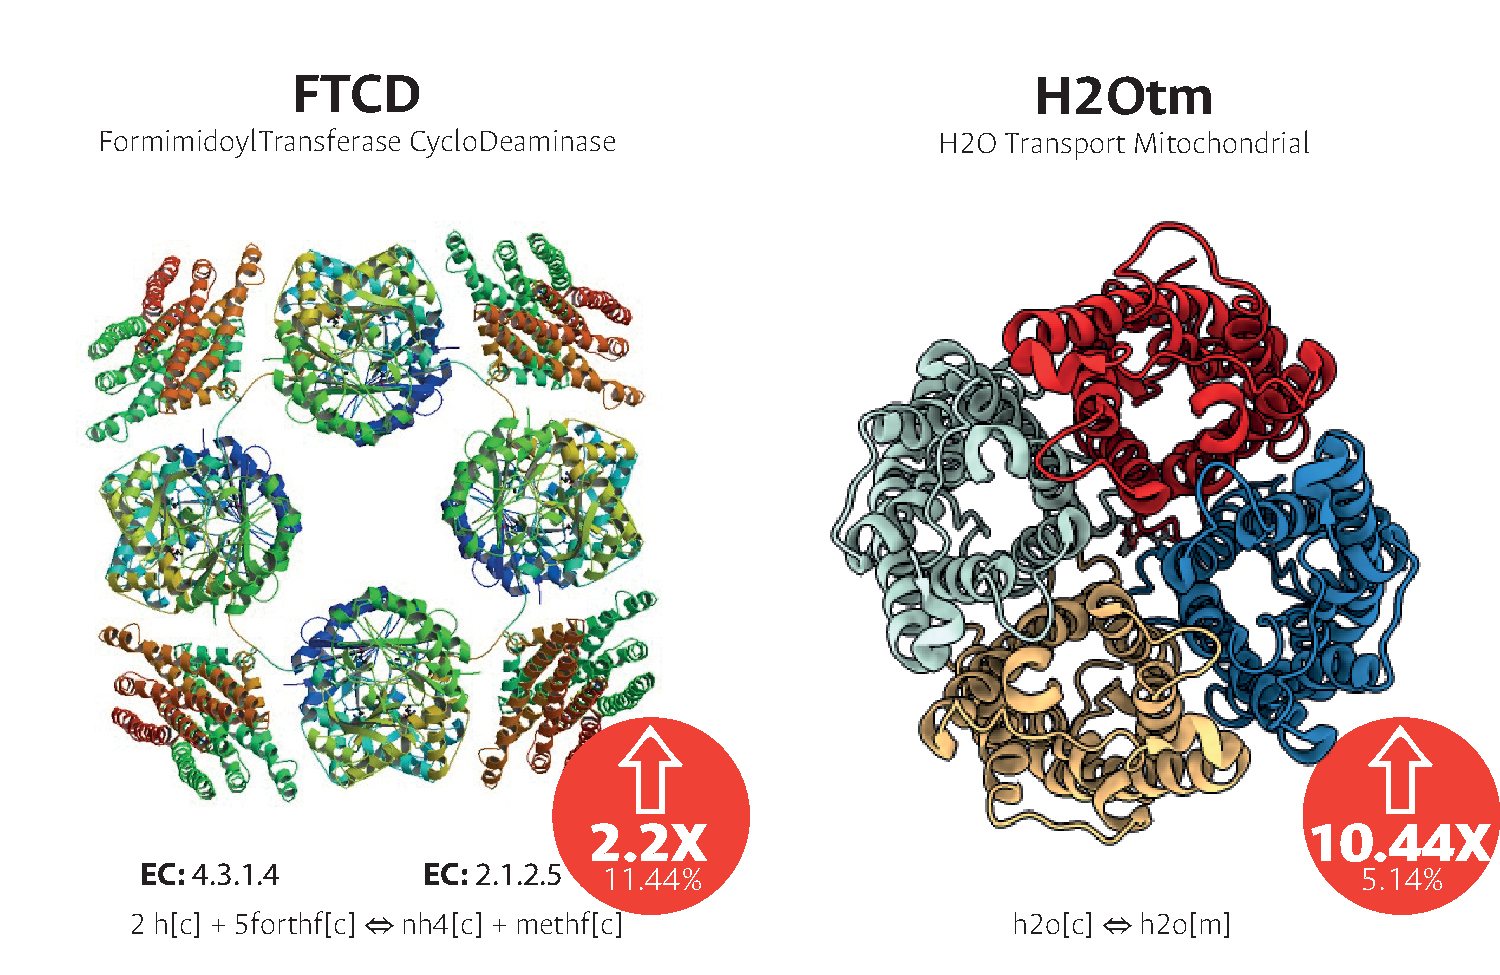
\includegraphics[width=\textwidth]{ProInflammatory}
\end{center}
\end{frame}
\begin{frame}{74 Anti inflammatory Enzymes}
\begin{center}
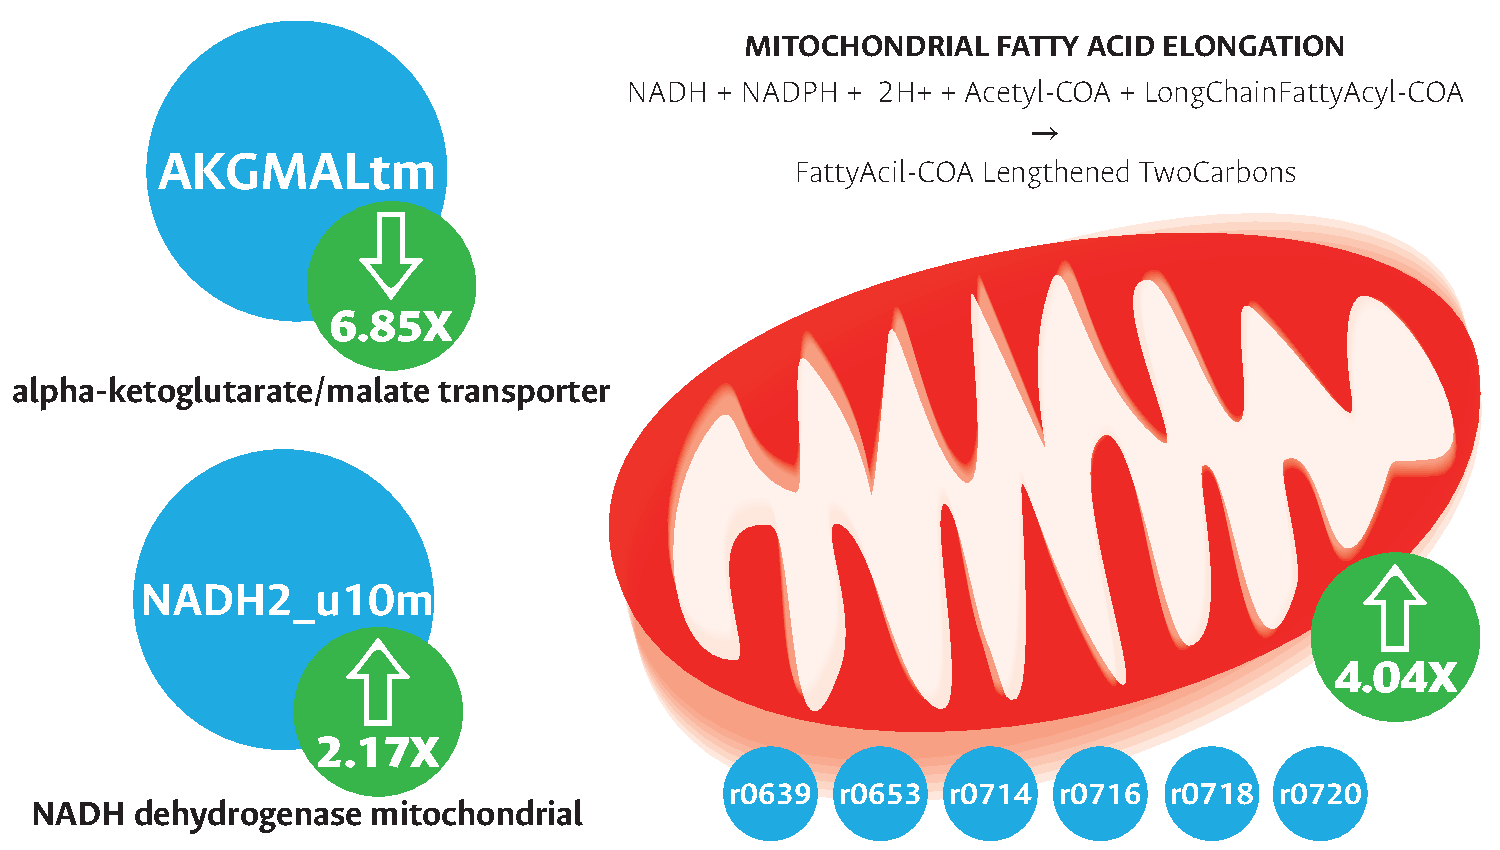
\includegraphics[width=\textwidth]{Antiinflammatory}
\end{center}
\end{frame}
\begin{frame}{Tibolone Related Enzymes}
\begin{center}
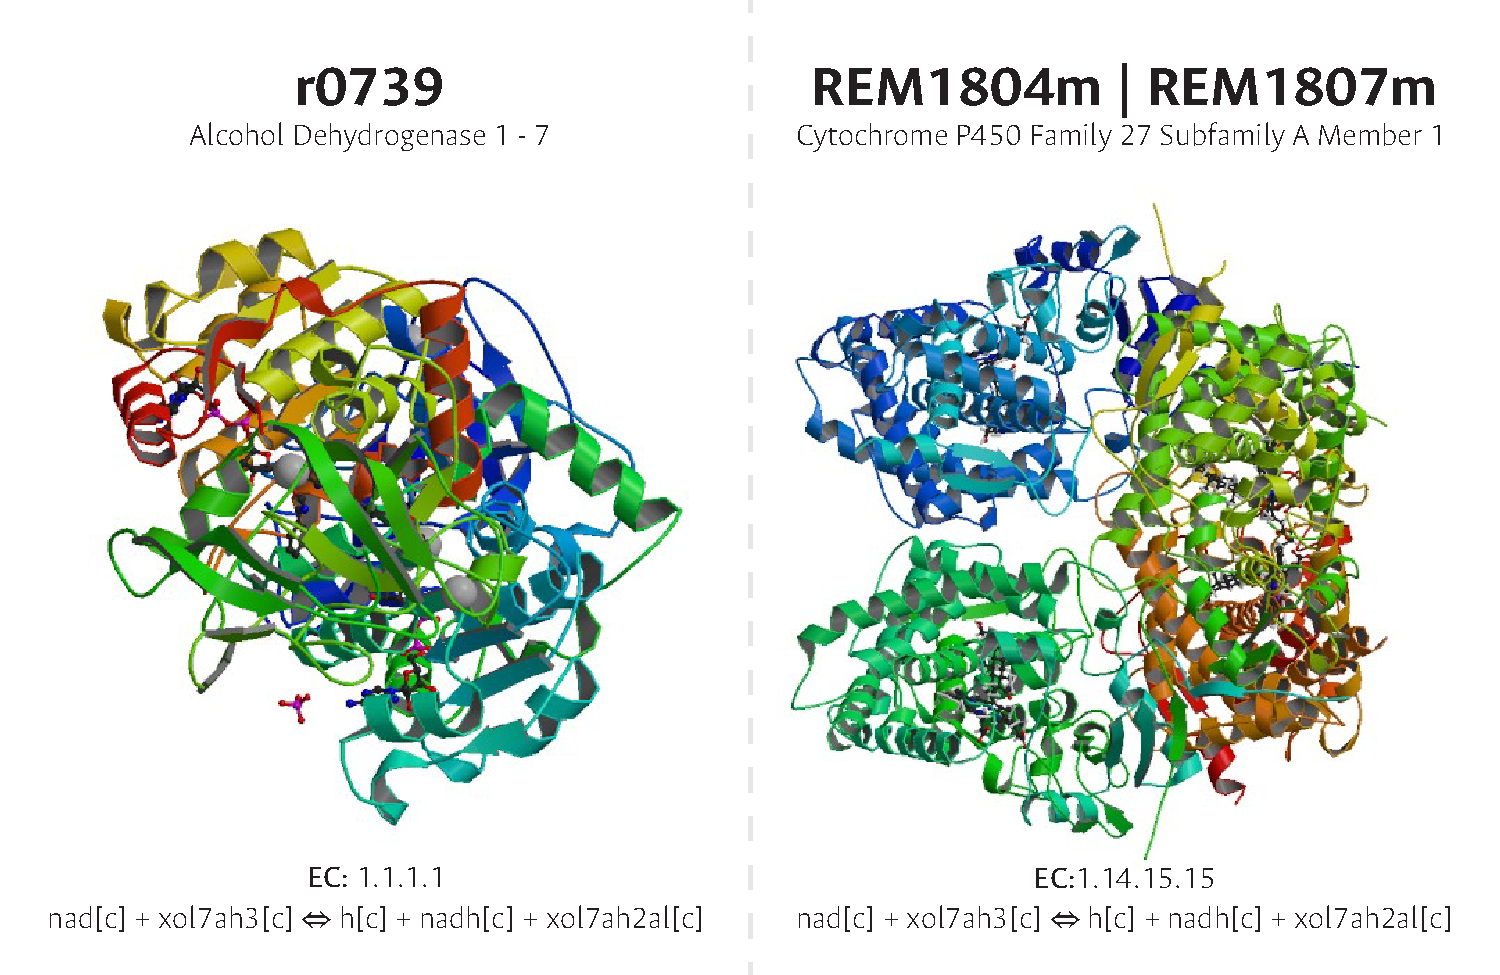
\includegraphics[width=\textwidth]{TiboloneEnzymes}
\end{center}
\end{frame}
\section{Conclusions}
\begin{frame}
\begin{center}

\end{center}
\end{frame}
\section{Events}
\begin{frame}{Advances of this work were presented as:}
\begin{center}
\includegraphics[width=\textwidth]{Events}
\end{center}
\hrulefill \ at: \hrulefill
\begin{multicols}{3}
\begin{center}
\includegraphics[width=0.3\textwidth]{IS3B}\\
CDMX, México\\
\textbf{Short Talk}
\end{center}
\begin{center}
\includegraphics[width=0.3\textwidth]{ICSB}\\
Barcelona, España\\
\textbf{Poster}
\end{center}
\begin{center}

\includegraphics[width=0.3\textwidth]{ICGEB}\\
Bogotá, Colombia\\
\textbf{Short Talk}
\end{center}
\end{multicols}
\end{frame}
\section{Acknowledgements}
\begin{frame}{Acknowledgements}

\end{frame}
\section{Questions}
\begin{frame}{This study was developed at the:}
\begin{multicols}{2}
\includegraphics[height=0.7cm]{logoIG}
\begin{flushright}
\includegraphics[height=0.7cm]{logoGIBBS}
\end{flushright}
\end{multicols}
\begin{center}
\includegraphics[width=\textwidth]{GIBBS}\\
\textbf{Bioinformatics and Computational Systems Biology Lab}\\
Institute for Genetics - Universidad Nacional de Colombia
\end{center}
\begin{center}
\textbf{CONTACT:}
\begin{multicols}{2}
\begin{center}
\textbf{Daniel Osorio}\\
dcosorioh@unal.edu.co\\
\textbf{Andrés Pinzón PhD}\\
ampinzonv@unal.edu.co
\end{center}
\end{multicols}
\end{center}
\end{frame}
\end{document}
